\documentclass[../main.tex]{subfiles}
\begin{document}

\section{Signal extraction}
\label{hh:sec:signal_extraction}

% The eight orthogonal categories described in Section~\ref{hh:sec:event_categorization} are used for the signal extraction via a DNN developed to identify \hhbbtt{} events.


To perform the signal extraction, a different DNN was developed in order to identify \hhbbtt{} events. The approach used to train this DNN \cite{hh:analysis:gilesdnn} follows the one used in the CMS di-Higgs HL-LHC projection analysis for the bb$\tau\tau$ channel \cite{hh:analysis:hh_hllhc}. The goal of the DNN is to classify events as originating either from signal (SM \hhbbtt{} produced via ggF) or background processes by assigning to them a single prediction score. Score values closer to one indicates ``signal-like'' events, while  closer to zero, ``background-like'' events. The final DNN distributions obtained by inferring this network prediction in each category, $\tau\tau$ decay channel and year are used in the signal extraction fit.

Training is performed with the \textsc{PyTorch} \cite{hh:analysis:pytorch} algorithm interfaced with \textsc{LUMIN} \cite{hh:analysis:lumin} using all MC-driven backgrounds as background processes and SM HH~$\to$~bb$\tau\tau$ as signal. Simulated events used for training are split in two halves, the ones with even event number and the ones with odd event number. A pair of discriminators are then trained with each half of the data. At inference time, the discriminators are used to predict the classes of events in the complementary halves of the data, i.e. the one trained with even event numbers for the odd event numbers, and vice versa. This way, all MC data can be used for the training without adding a bias on the predictions that would arise if only one network was used and the same data used for training was also used for inference. To further increase the statistical robustness, each discriminator consists of 10 neural networks, each trained with a different starting random seed.

For the training, a total of 26 features (selected among over a 100) are used as input to the neural network. Both categorical (year of data taking, the $\tau\tau$ decay mode or the number of VBF jet candidates) and object features are used. From the latter, the most important features (ranked by permutation importance) are the DeepJet scores of the b jets, the invariant masses of the bb, $\tau\tau$, and HH systems and kinematic variables of the reconstructed particles. The distributions of the masses of the bb, $\tau\tau$, and HH systems are shown in Fig.~\ref{hh:fig:dist_1} and \ref{hh:fig:dist_2} in four analysis categories: Resolved, 1 b-tag and 2 b-tag, Boosted, and VBF inclusive. The three years from Run 2 data taking and the three $\tau\tau$ decay channels are displayed together in each distribution. Each plot shows the data, the background contributions and two SM signals, HH ggF and VBF, scaled so their maximum is close to the one from the sum of backgrounds. All corrections described in Section~\ref{hh:sec:corrections} have been applied to the simulated events. In all distributions, there is a good agreement between the data and the backgrounds, in general within the statistical uncertainty ranges.



\subsection{VBF signal extraction}

After the development of the DNN devoted to signal extraction and the multi-class classification strategy for VBF analysis, a complete study was performed in order to determine the signal extraction strategy for the VBF signal. Four different strategies were proposed:


\begin{figure}[p!]
\begin{center}
\subfloat{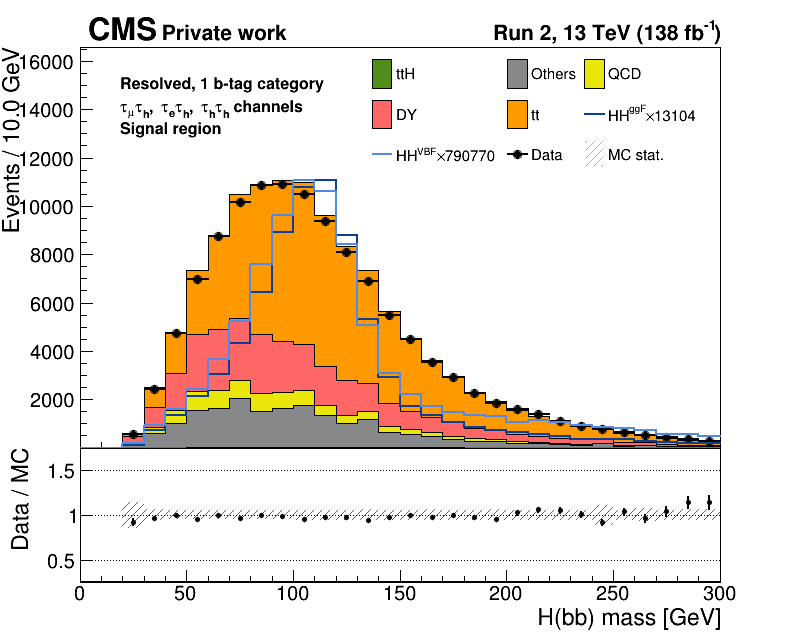
\includegraphics[width=0.49\textwidth]{Images/controlplots/bh_m_resolved_1b.pdf}}
\subfloat{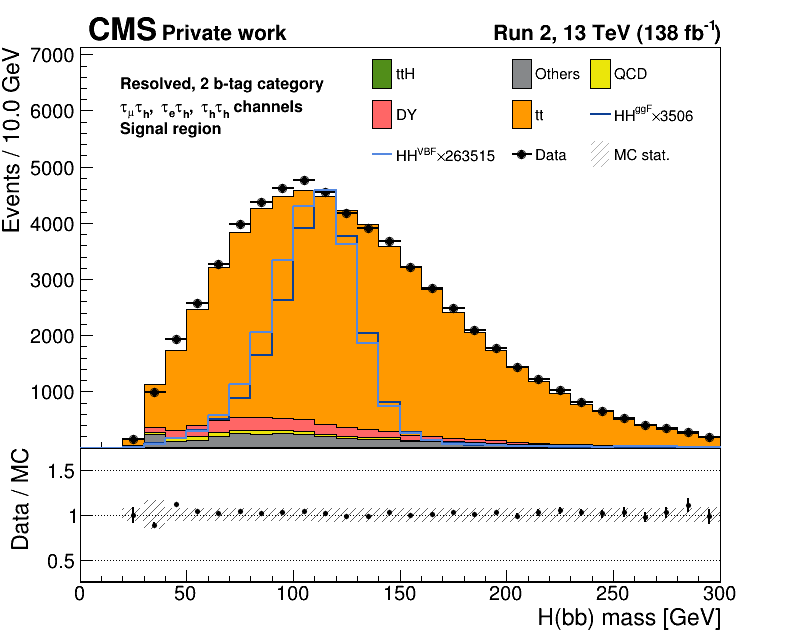
\includegraphics[width=0.49\textwidth]{Images/controlplots/bh_m_resolved_2b.pdf}}\\
\subfloat{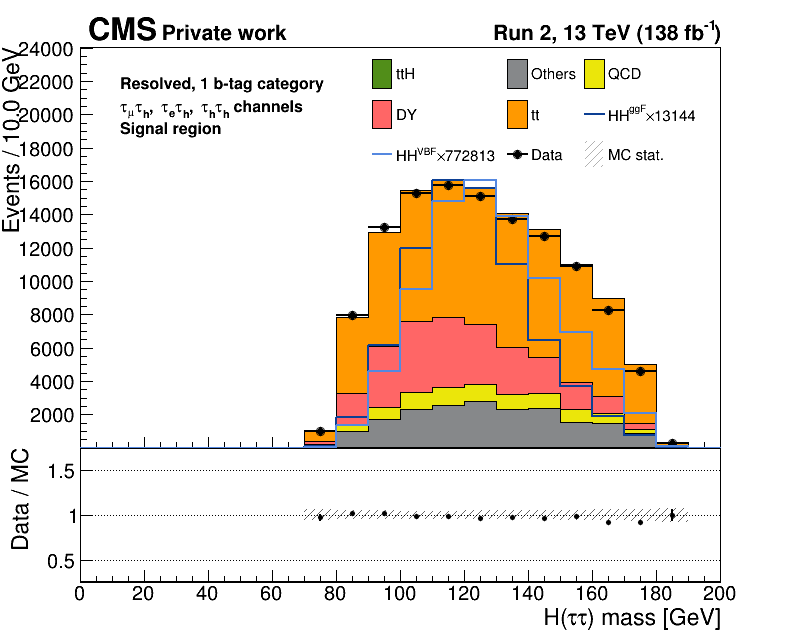
\includegraphics[width=0.49\textwidth]{Images/controlplots/tauh_sv_m_resolved_1b.pdf}}
\subfloat{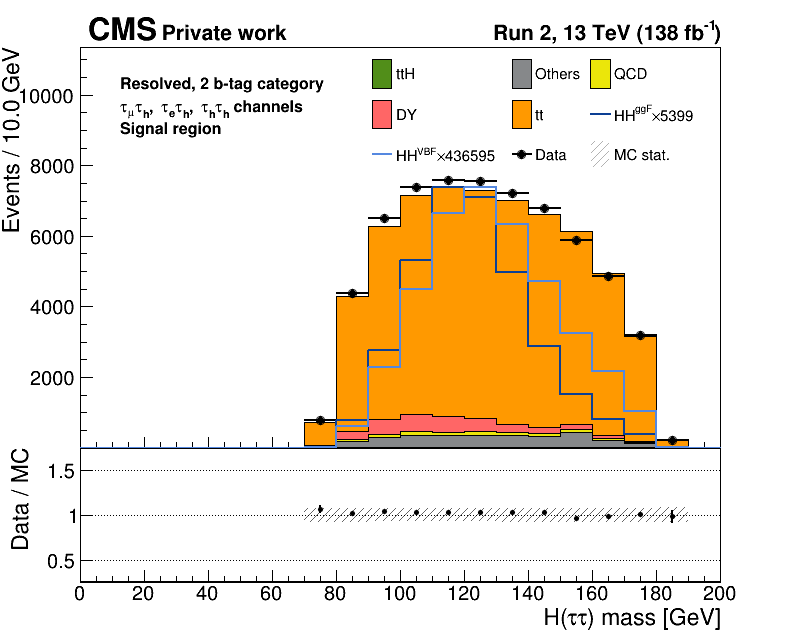
\includegraphics[width=0.49\textwidth]{Images/controlplots/tauh_sv_m_resolved_2b.pdf}}\\
\subfloat{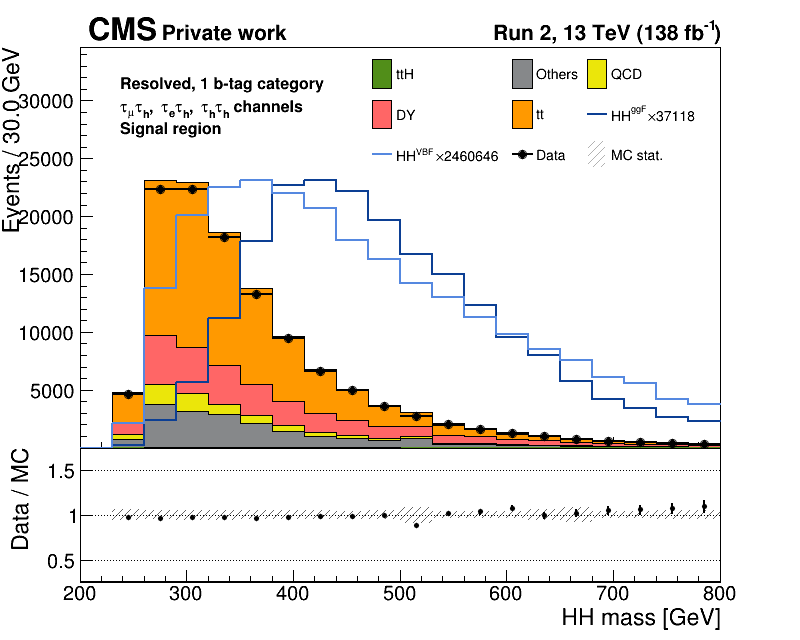
\includegraphics[width=0.49\textwidth]{Images/controlplots/hh_m_kin_resolved_1b.pdf}}
\subfloat{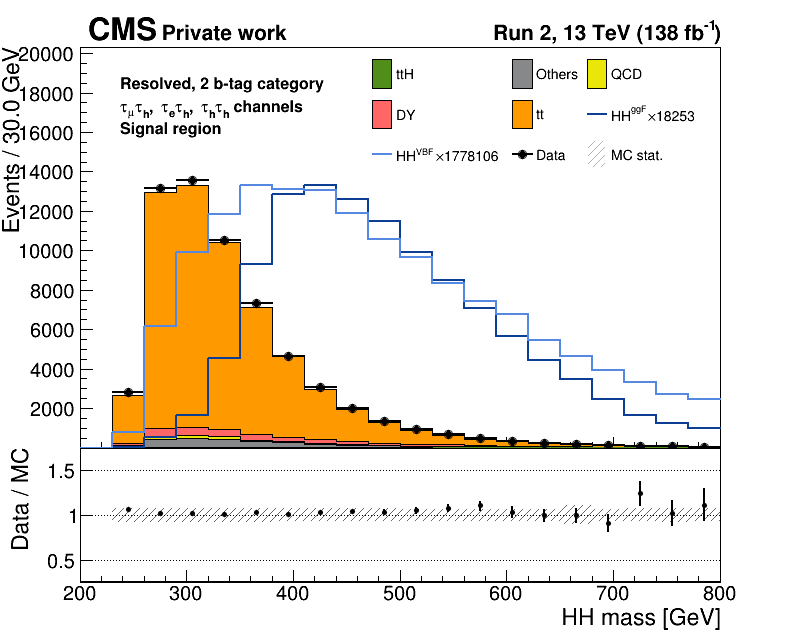
\includegraphics[width=0.49\textwidth]{Images/controlplots/hh_m_kin_resolved_2b.pdf}}\\
\end{center}
\caption[Mass distributions in the resolved categories in 2018]{Distributions of the masses of the H~$\to$~bb candidate (top), H~$\to\tau\tau$ candidate (middle), and HH system (bottom) for the Resolved, 1 b-tag (left), and Resolved, 2 b-tag (right) analysis categories. Each distribution contains the full Run 2 data sets and the three $\tau\tau$ decay channels.}
\label{hh:fig:dist_1}
\end{figure}

\begin{figure}[p!]
\begin{center}
\subfloat{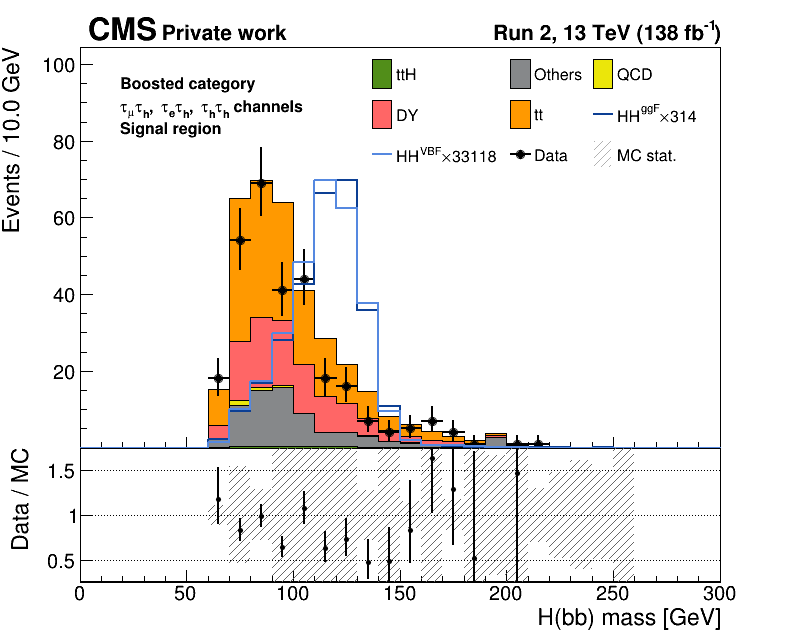
\includegraphics[width=0.49\textwidth]{Images/controlplots/bh_m_boosted.pdf}}
\subfloat{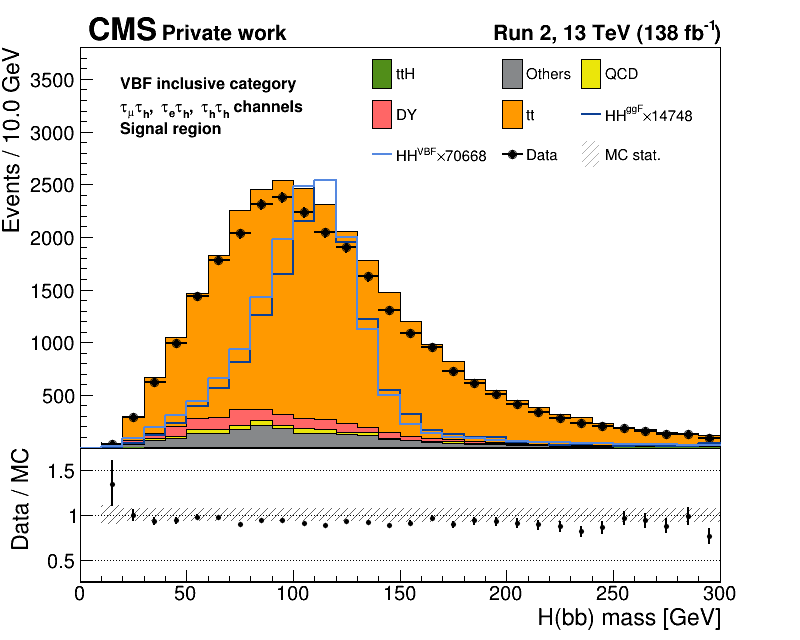
\includegraphics[width=0.49\textwidth]{Images/controlplots/bh_m_vbf.pdf}}\\
\subfloat{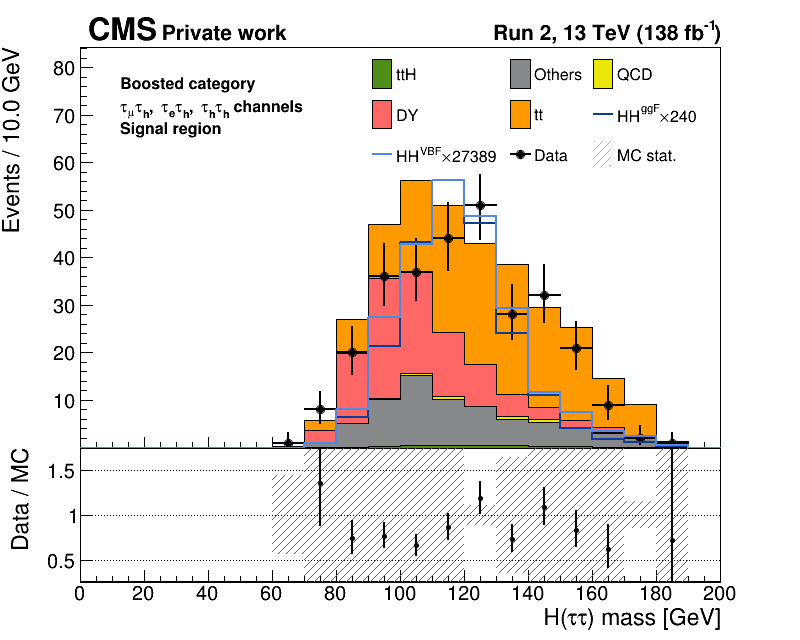
\includegraphics[width=0.49\textwidth]{Images/controlplots/tauh_sv_m_boosted.pdf}}
\subfloat{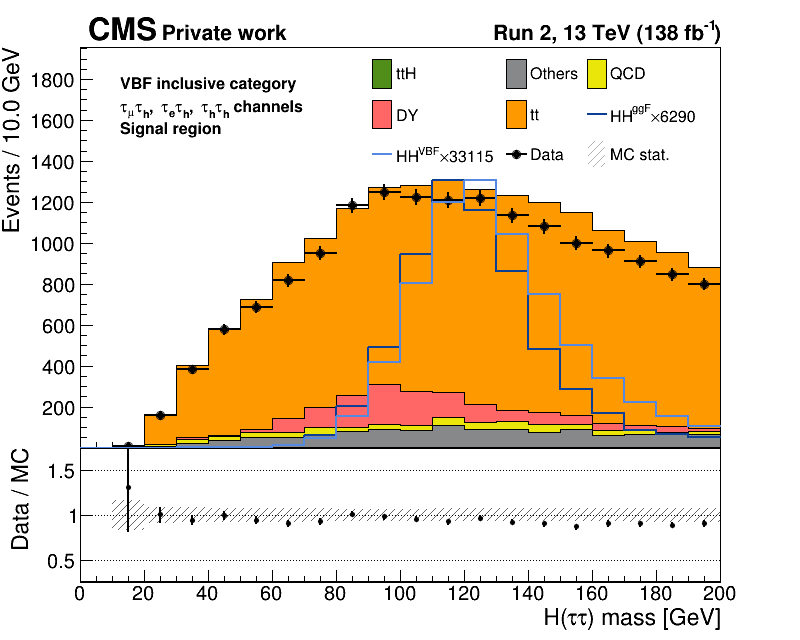
\includegraphics[width=0.49\textwidth]{Images/controlplots/tauh_sv_m_vbf.pdf}}\\
\subfloat{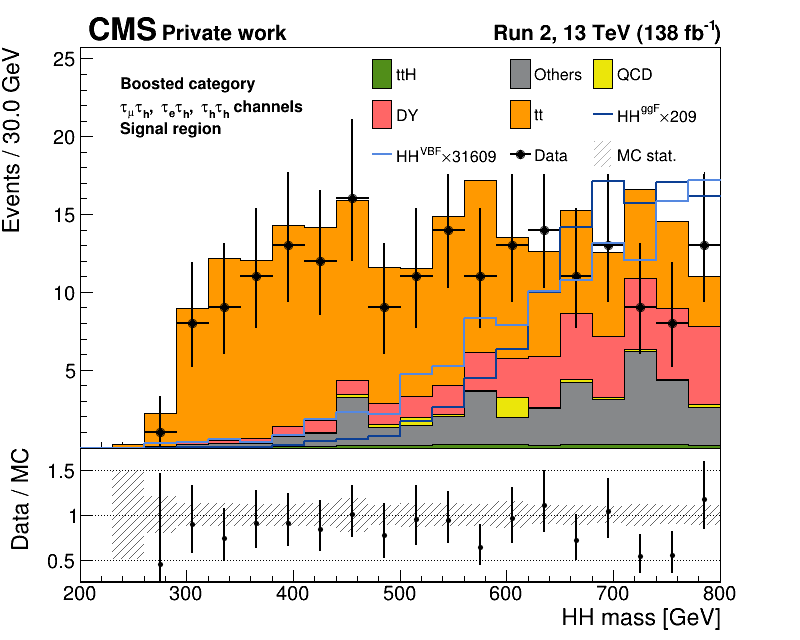
\includegraphics[width=0.49\textwidth]{Images/controlplots/hh_m_kin_boosted.pdf}}
\subfloat{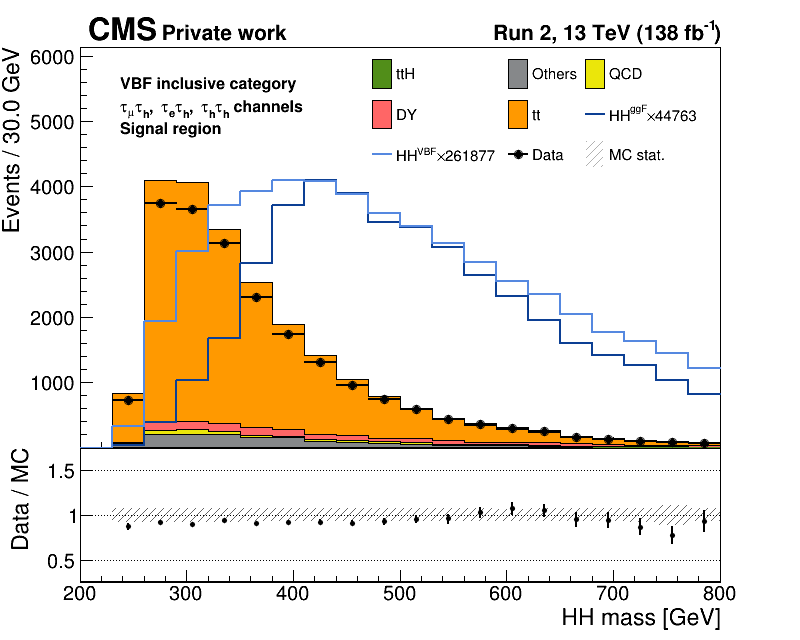
\includegraphics[width=0.49\textwidth]{Images/controlplots/hh_m_kin_vbf.pdf}}\\
\end{center}
\caption[Mass distributions in the boosted and VBF inclusive categories in 2018]{Distributions of the masses of the H~$\to$~bb candidate (top), H~$\to\tau\tau$ candidate (middle), and HH system (bottom) for the Boosted (left), and VBF inclusive (right) analysis categories. Each distribution contains the full Run 2 data sets and the three $\tau\tau$ decay channels.}
\label{hh:fig:dist_2}
\end{figure}

\begin{enumerate}
	\item Consider the output score of the VBF node from the multi-class classification approach in the VBF inclusive category.
	\item Consider the signal extraction DNN (from now onwards, DNN) output score in the VBF inclusive category, i.e. avoid using the multi-class classification approach.
	\item Consider the output score of the VBF node from the multi-class classification approach but splitting the VBF inclusive category into five subcategories defined by the processes considered in the multi-class classification: HH ggF, HH VBF, \ttbar{}, \tth, and \dyjets{}. Events are categorised by selecting the process whose corresponding node obtained the highest value.
	\item Consider the DNN output score in the five VBF subcategories.
\end{enumerate}

The output score in the categories defined by the different strategies is shown in Fig.~\ref{hh:fig:vbf_signal_extraction} (in strategies 3. and 4., only the output score in the HH VBF subcategory is displayed, as it should give the largest sensitivity in the VBF analysis). Some observations can be extracted from this Figure:
\begin{itemize}
	\item The DNN output score from the HH VBF process is contained mostly in the last bin from the distributions, where the background event yield is the smallest. The output score of the VBF node is more uniformly distributed (although mostly contained in the last bins of the distributions).
	\item The categorisation strategy defined by the multi-class classification approach helps drastically reducing the amount of background in the category, which could provide more sensitivity.
\end{itemize} 

\begin{figure}[h!]
\begin{center}
\subfloat{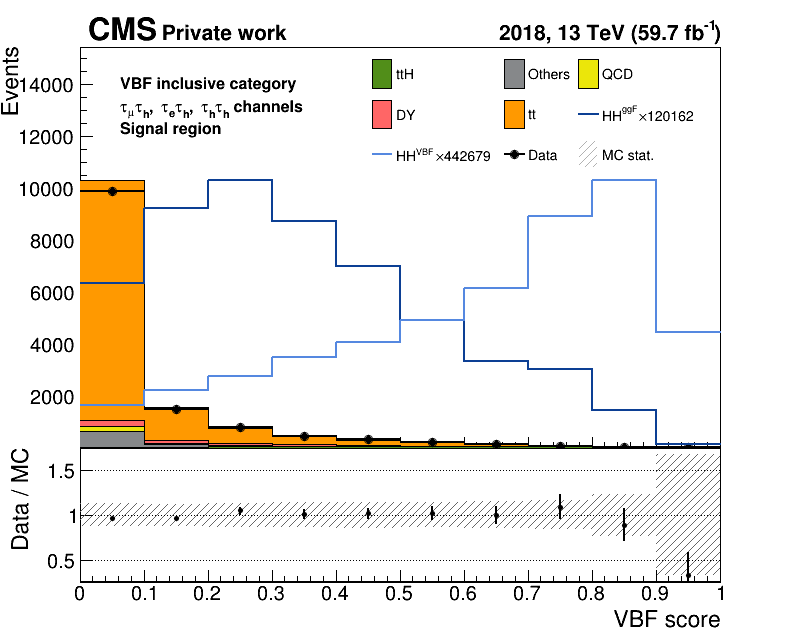
\includegraphics[width=0.49\textwidth]{Images/controlplots/dnn_hh_vbf_sm_c2v_merged_vbf.pdf}}
\subfloat{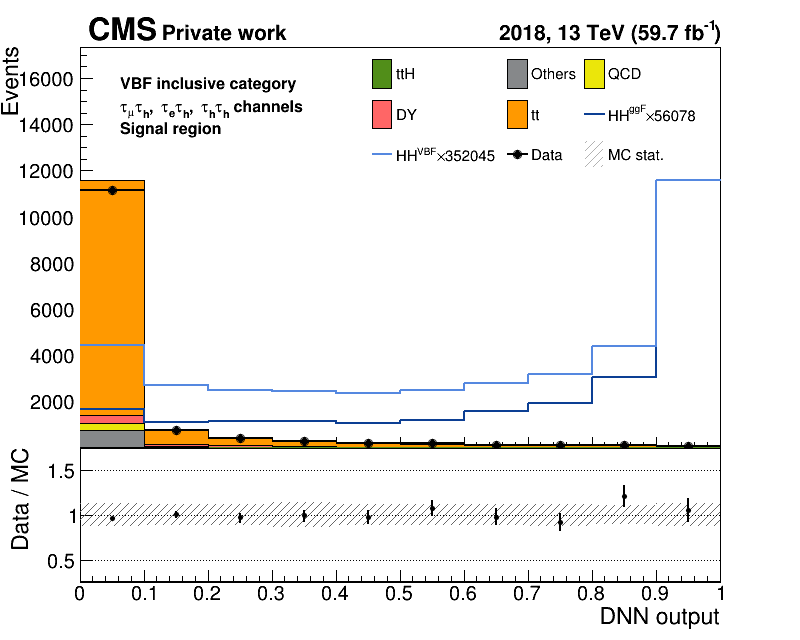
\includegraphics[width=0.49\textwidth]{Images/controlplots/DNNoutSM_kl_1_vbf.pdf}}\\
\subfloat{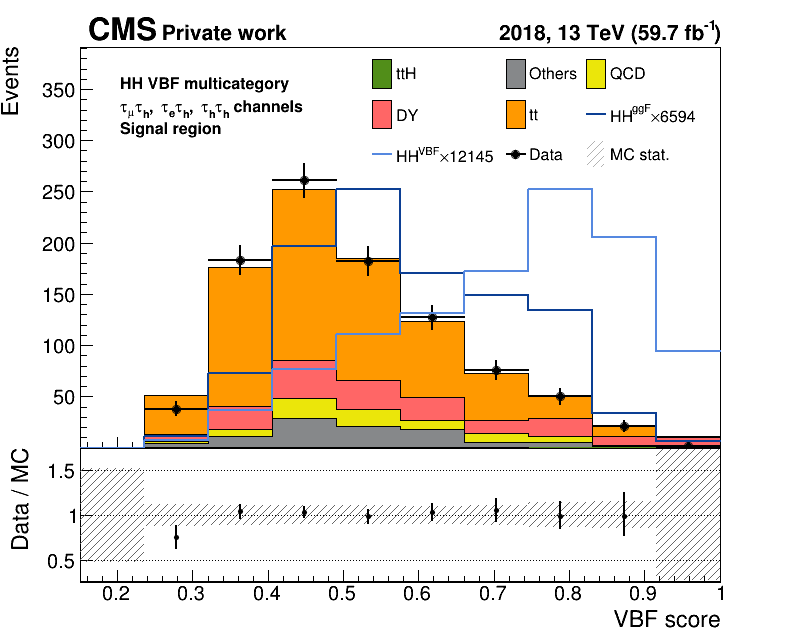
\includegraphics[width=0.49\textwidth]{Images/controlplots/dnn_hh_vbf_sm_c2v_merged_mpp_vbf.pdf}}
\subfloat{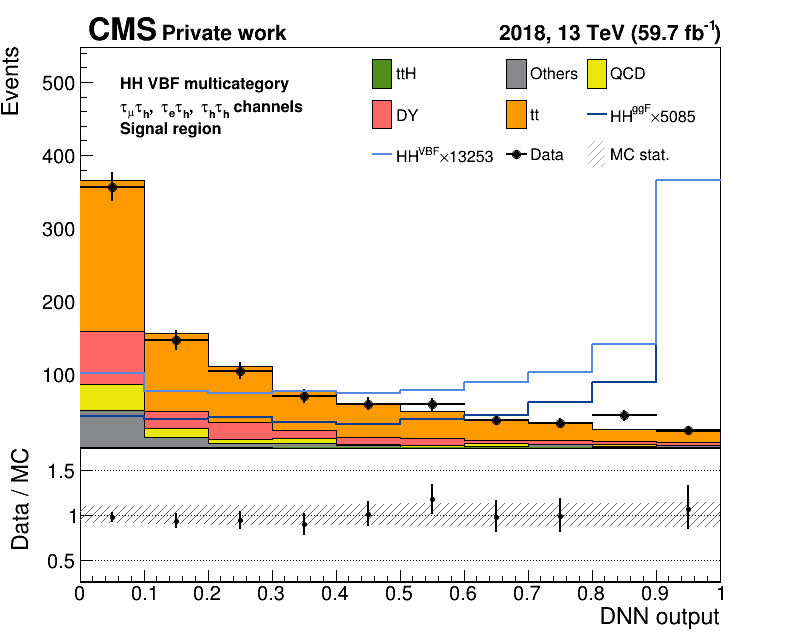
\includegraphics[width=0.49\textwidth]{Images/controlplots/DNNoutSM_kl_1_hh_vbf_sm_c2v_merged_mpp_vbf.pdf}}\\
\end{center}
\caption[Output scores for the different VBF signal extraction strategies]{Distributions of the output score of the VBF node in the VBF inclusive category (top left) and the HH VBF subcategory (bottom left) and distributions of the DNN output score in the VBF inclusive category (top right) and the HH VBF subcategory (bottom right). Results are shown for 2018 and the three $\tau\tau$ decay channels together.}
\label{hh:fig:vbf_signal_extraction}
\end{figure}

In order to estimate the sensitivity that could be provided by the four strategies described, the binned significance is considered, obtained as the ratio between the signal yield (in this case, HH VBF) and the square root of the total background yield in a particular bin. With this binned significance, two quantities are used to measure the sensitivity: the maximum binned significance over all bins in the distribution and the sum of the binned significances from all bins. The higher their values, the more sensitivity the distribution should provide. The values obtained for 2018 split by $\tau\tau$ decay are shown in Table~\ref{hh:tab:vbf_sensitivity}. In general, the largest values are obtained by the fourth strategy, i.e. the DNN output score obtained in the subcategories defined by the multi-class classification approach. In fact, only the HH VBF is considered here, but the other subcategories could also provide more sensitivity: some signal could be allocated in the HH ggF subcategory, and the background subcategories could help constraining the values of the systematic uncertainties.

In conclusion, the DNN developed for signal extraction will be used in the eight orthogonal categories (Resolved 1 b-tag, Resolved 2 b-tag, Boosted and the five VBF subcategories).


\begin{table}[h!]
\begin{footnotesize}
\begin{tabular}{l|rr|rr|rr}
& \multicolumn{2}{c|}{$\tau_\mu\tau_h$ channel}
& \multicolumn{2}{c|}{$\tau_e\tau_h$ channel}
& \multicolumn{2}{c}{$\tau_h\tau_h$ channel}
\\
\cline{2-7}
& $\max_i S_i/\sqrt{B_i}$ & $\sum_i S_i/\sqrt{B_i}$
& $\max_i S_i/\sqrt{B_i}$ & $\sum_i S_i/\sqrt{B_i}$
& $\max_i S_i/\sqrt{B_i}$ & $\sum_i S_i/\sqrt{B_i}$ \\
\hline
Strategy 1 & 0.0022 & 0.0072 & 0.0021 & 0.0067 & 0.0054 & 0.0157 \\
Strategy 2 & 0.0025 & 0.0056 & 0.0017 & 0.0038 & 0.0061 & 0.0137 \\
Strategy 3 & 0.0020 & 0.0073 & 0.0018 & 0.0068 & 0.0049 & 0.0164 \\
Strategy 4 & 0.0036 & 0.0085 & 0.0025 & 0.0060 & 0.0139 & 0.0244
\end{tabular}
\end{footnotesize}
\caption[Maximum binned significance results for VBF signal extraction]{Values obtained for the maximum binned significance and the sum of binned significances for the distributions defined by the four VBF signal extraction strategies. Results are obtained using 2018 data and the three $\tau\tau$ decay channels separately.}
\label{hh:tab:vbf_sensitivity}
\end{table}



\end{document}

